\documentclass[../summary.tex]{subfiles}

\begin{document}
\section{Raw materials and circular economy}
\subsection{Introduction}	
\subsubsection{What are resources}
	
Our prosperity relies on easy access to abundant raw materials, with global demand exceeding 100 billion tonnes annually and predicted to double by 2060. Raw materials, substances or resources processed for product creation, are sourced from the earth's crust, nature, and recycled waste in the economy or technosphere. \\
\\
Examples of raw materials from the lithosphere or earth crust are fossil oil and gas, iron ore, bauxite as raw material for aluminium, minerals such as sand or marble, lithium brines, and so on. Metals are often found in ores with varying concentrations, and their distribution is uneven globally. Biomass, derived from nature, includes plant-based and animal-derived materials. Secondary raw materials, extracted from recycled waste, vary in extraction rates, e.g., lead at 70\%, while lithium remains below 1\%. Despite recycling efforts, 88 to 94\% of materials in new products still come from primary resources. \\
\\
Raw material sources span the litho-, bio-, and technosphere. The industrial metabolism concept likens the economy's material processes to the human body's metabolism, providing insight into material management, waste, and emissions for sustainable improvements.

\subsubsection{Case: Electric car}

The ongoing effort to combat climate change includes a significant focus on the energy transition, with a key aspect being the widespread adoption of electric vehicles (EVs). The transition is evident in the rapid increase in EV sales, accounting for 14\% of new car sales in 2022, up from 9\% in 2021 and 5\% in 2020. Figure \ref{fig:electriccarsales} depicts a substantial rise in electric car sales, reaching an estimated 14 million in 2023, with 8 million sold in China.

\begin{figure}[H]
	\centering
	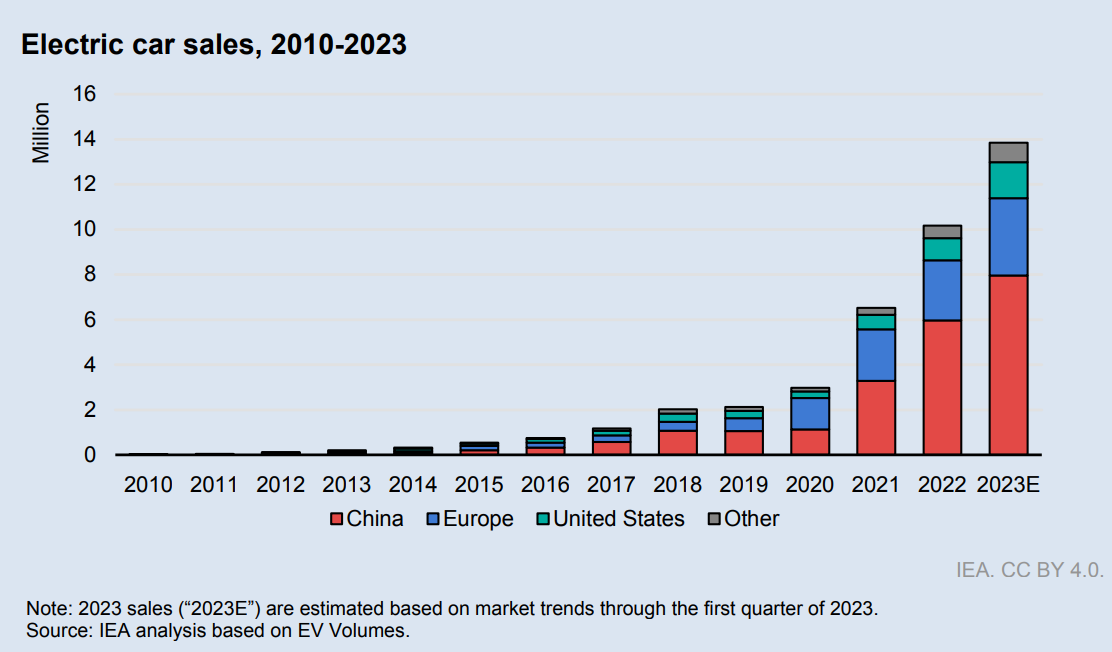
\includegraphics[width=0.7\linewidth]{../images/Electric_car_sales}
	\caption{Electric car sales between 2010 and 2023}
	\label{fig:electriccarsales}
\end{figure}
\ \\
The shift to EVs brings about a change in the materials used, replacing combustion engines with catalysts containing Pt, Pd, and Rh with electric motors requiring copper and neodymium magnets (NdFeB). Power is supplied by Li-ion batteries, raising concerns about the availability of materials to meet the growing demand. Questions arise regarding the duration of lithium availability for Li-ion batteries and the overall environmental impact of EVs compared to traditional combustion engine vehicles. Additionally, considerations about battery recycling and recyclability play a crucial role in evaluating the sustainability of electric vehicles.

\subsection{Material demand}
\subsubsection{trends in material demand}

Over the past five decades, global demand for materials has surged, more than tripling, outpacing both population and GDP growth. While the world's population doubled during this period, the \textbf{gross domestic product} (GDP) quadrupled. The implications of this growth raise questions about the future trajectory of our material needs over the next 10, 20, or 100 years. To forecast this trajectory, an analysis of the driving forces behind the evolution of global material demand is crucial.\\
\\
Three primary factors propel global material demand: population, affluence (which represents the average level of wealth per person, measured by GDP per capita), and technology (material intensity per dollar of GDP). While population growth continues, its significance in driving material demand is diminishing due to declining growth rates. Affluence, reflecting individual wealth, has seen a consistent growth rate when adjusted for inflation and cost of living, leading to a stable projection for the foreseeable future.\\
\\
The most intricate factor, technology, involves examining the material efficiency of the economy. Comparisons between GDP per person and material footprint per person across countries reveal a trend – larger GDP correlates with a larger material footprint, but the relationship is not strictly linear. This observation holds true over the years, suggesting a pattern in global evolution.\\
\\
In industrialized nations, a notable trend emerges – a relative decoupling of economic growth and material demand growth. While the absolute material footprint increases, the relative footprint per dollar of GDP decreases. This pattern contrasts with countries undergoing industrialization, such as China in the past 30 years, where material demand grew faster than GDP due to intense infrastructure development.\

\begin{figure}[H]
	\centering
	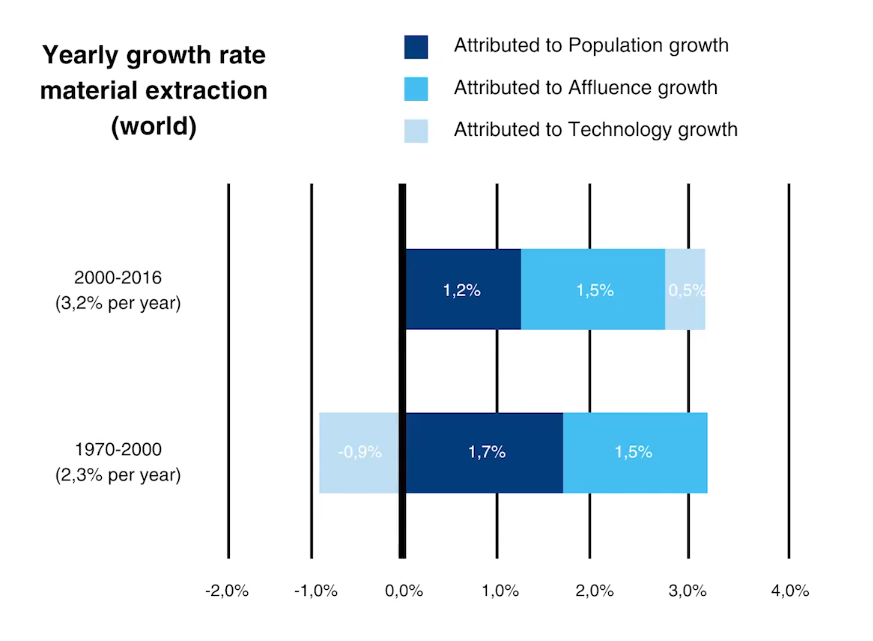
\includegraphics[width=0.7\linewidth]{../images/material_demand_growth_rates}
	\caption{Material demand growth rates throughout the past 50 years}
	\label{fig:materialdemandgrowthrates}
\end{figure}
\ \\
Looking ahead, the future trajectory involves anticipating the dynamics of these three factors. Population growth will continue but at a slower pace. Affluence will persist in its growth to ensure equal opportunities globally. The technology factor, representing material intensity, is expected to vary across countries. China, a significant purchaser of materials, is forecasted to enter a less material-intensive phase, while countries like India and many African nations may undergo material-intensive development phases.\\
\\\\
The Organisation for Economic Co-operation and Development (OECD) foresees a doubling of worldwide material demand by 2060, indicating further growth. However, this growth will not be uniform across all material types. Materials crucial for the energy transition, such as lithium, are expected to experience much higher growth rates. For instance, demand for lithium in 2050 is projected to be 20 times higher than today, emphasizing the changing landscape of material needs in the context of evolving technologies and global priorities.

\subsubsection{Case: Electric car}

The shift towards electrical mobility requires a lot of materials that where not very much used before, such as Lithium, and an substantial increase in demand of some commodities, such as Nickel or Copper. Figure \ref{fig:Lithium} and \ref{fig:Nickel} underneath show the forecasted demand for the coming decades of lithium and nickel, in the case of the STEPS and SDS IEA scenarios.

\begin{figure}[H]
	\centering
	\begin{subfigure}{.5\textwidth}
		\centering
		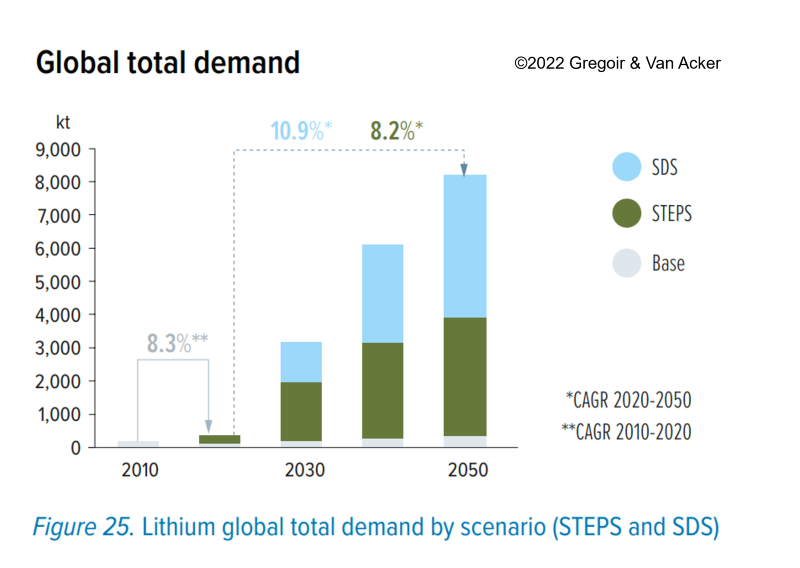
\includegraphics[width=1\linewidth]{../images/Global_lithium_demand_STEPS_SDS}
		\caption{Lithium}
		\label{fig:Lithium}
	\end{subfigure}%
	\begin{subfigure}{.5\textwidth}
		\centering
		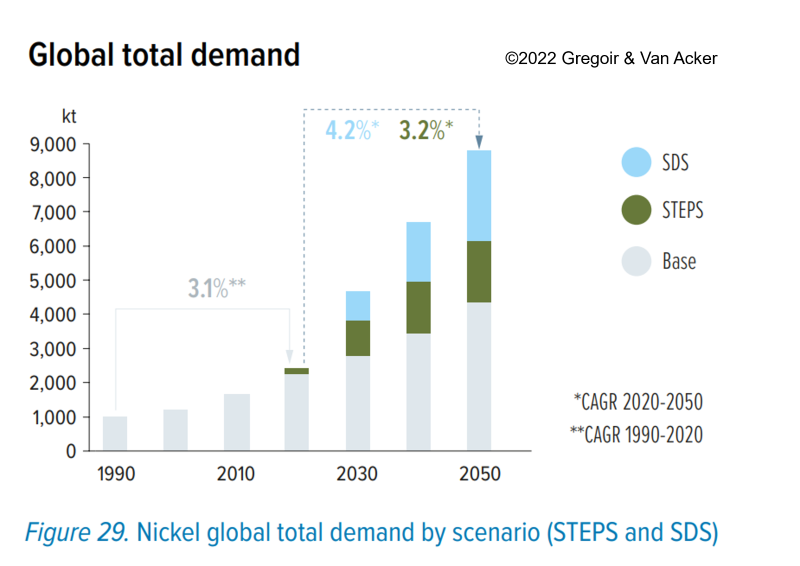
\includegraphics[width=1\linewidth]{../images/Global_nickel_demand_STEPS_SDS}
		\caption{Nickel}
		\label{fig:Nickel}
	\end{subfigure}
	\caption{Global total demand by STEPS  and SDS scenarios}
	\label{fig:Global total demand}
\end{figure}
\ \\
Two scenarios as put forward by the International Energy Agency are considered in these figures:\\
\\
\textbf{The Stated Policies Scenario (STEPS) }reflects current policy settings based on a sector-by-sector assessment of the specific policies that are in place, as well as those that have been announced by governments around the world. It provides an indication of where today’s policy measures and plans lead the energy sector.\\
\\
\textbf{The Sustainable Development Scenario (SDS) }charts a pathway that meets in full the world’s goals to tackle climate change in line with the Paris Agreement while meeting universal energy access and significantly reducing air pollution. In this scenario, all current net zero pledges are achieved in full and there are extensive efforts to realize near-term emissions reductions; advanced economies reach net zero emissions by 2050, China around 2060, and all other countries by 2070 at the latest.
\newpage
\subsection{Material scarcity}
\subsubsection{Causes of scarcity}

The availability of materials is a nuanced issue that involves various dimensions of scarcity. Examining the abundance of chemical elements in the Earth's crust reveals disparities, with some elements being plentiful, such as silicon and aluminium, while others, like gold, are rare but economically interesting to mine due to the concentration in ores.\\
\\
Absolute scarcity, often associated with the idea of running out of resources, is challenging to predict due to ongoing exploration and technological advancements enabling the extraction of materials from less concentrated ores. However, significant challenges exist in terms of depleting easily accessible and high-quality raw materials, with quality meaning the concentration of useful elements the raw materials contain. For instance, copper ore quality has decreased over time from 3\% to 0,3\%, necessitating larger amounts to be mined for the same output.\\
\\
Another dimension of scarcity involves the geopolitical and economic concentration of certain ores in specific countries. This concentration, as seen with lithium in Bolivia, Chile, and Argentina, cobalt in Central and South Africa, and rare earth metals in China, can lead to global supply chain vulnerabilities, especially when geopolitical tensions arise.\\
\\
Additionally, some high-tech elements, like indium which is found in zinc, are structurally scarce as they are by-products of ores containing more abundant metals. This linkage can create challenges in meeting demand, as increasing production of the desired element may flood the market with the carrier metal, affecting its price. Therefore, we say that indium is structurally scarce.\\
\\
In conclusion, while absolute scarcity is not imminent for most elements, the uneven distribution of ores, geopolitical and economic dependencies, and structural scarcity of certain elements pose significant challenges. Mitigating these challenges involves reducing dependence on raw materials, exploring alternative sources, and promoting sustainable practices to ensure a more resilient global economy.

\subsubsection{Case: Absolute scarcity}
\paragraph{Static and dynamic depletion index}
\ \\
Absolute scarcity describes the physical depletion of non-renewable resources. There is a certain amount available for extraction in reserves, but this amount will run out over time. When we want to predict how much time we have before a certain resource runs out, we look at the available reserve (R) and the yearly production or use of that resource (P).\\
\\
If we divide the current reserve by the current demand, so R/P, we see how many years are still left. This is called the static depletion index \textbf{static depletion index}. \\
\\
However, demand for raw materials changes, for most materials it increases. When we take the predicted change in demand into account, we call this the \textbf{dynamic depletion index}. For a resource with an increase in demand, the dynamic index will be smaller than the static index

\paragraph{Depletion of copper}
\ \\
The static and dynamic depletion indices for copper defy expectations, showing a relatively stable pattern over time instead of a continual decrease as assumed, as shown in figure \ref{fig:staticdynamicindexcopper}. This stability is attributed to the discovery of new reserves and advancements in extraction technology, prolonging the availability of copper. However, this prolonged use has consequences: the easily accessible copper ore has been depleted, leading to a decline in ore quality from 2-5\% copper at the beginning of the last century to 0.3\% today.
\newpage

\begin{figure}[H]
	\centering
	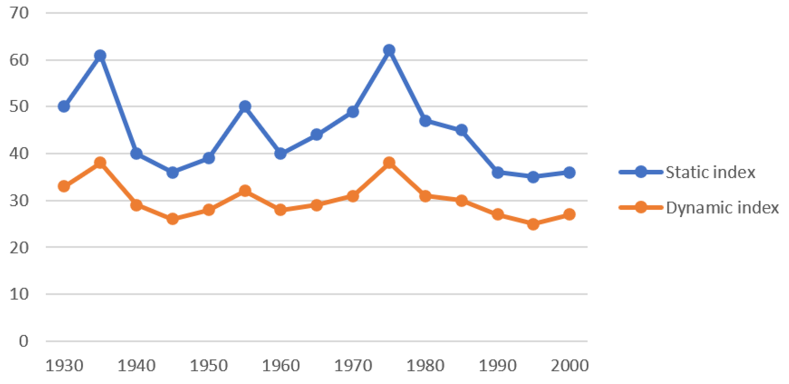
\includegraphics[width=0.7\linewidth]{../images/static_dynamic_index_copper}
	\caption{Static and dynamic index of Copper}
	\label{fig:staticdynamicindexcopper}
\end{figure}
\ \\
As a result:
\begin{itemize} 
	\item The need to mine ten times as much copper ore per kg of copper has increased.
	\item More energy is required to produce one kg of copper despite improved extraction technologies.
	\item The environmental impact is higher.
	\item The price of copper has risen, influenced by increased production costs and stricter environmental regulations.
\end{itemize}
\ \\
While predictions may initially suggest a resource is running out, the reality is an extended timeline with escalating costs and environmental impact.

\subsubsection{Case: Structural scarcity}

Materials that are structurally scarce, such as Germanium and Gallium, are primarily obtained as byproducts during the extraction of other materials.\\
\\
\textbf{Germanium}: It is derived mainly from sphalerite, found in ores of silver, lead, and copper. Another source is fly ash from coal-fueled power plants containing germanium. Germanium is utilized in optics (e.g., camera lenses, optical fibers, infrared cameras) and electronics (high-speed chips, solar panels).\\
\\
\textbf{Gallium}: Produced exclusively as a byproduct during the processing of other metal ores, with bauxite (chief ore of aluminum) and sulfidic zinc ores being primary sources. Gallium is employed in semiconductors (high-speed computer chips), photovoltaic cells, laser diodes, cable television transmission, commercial wireless infrastructure, and satellites.\\
\\
In addition to being structurally scarce, there can also be geopolitical scarcity. For instance, a significant portion of production occurs in China, which, in July 2023, announced export restrictions on specific gallium and germanium products. Fortunately, alternative sources for these minerals exist outside of China.
\newpage
\subsubsection{Case: Economic and geopolitical scarcity}

Price and availability of resources is also influenced by economics – supply and demand –and the geopolitical presence of the reserves. This is illustrated for example by cobalt. Cobalt is used in lithium batteries, which are used in electric vehicles. The main cobalt reserves are located in the east of Congo, a region which is politically unstable. \\
\\
Due to the climate crisis, there have been a lot of investments in electric vehicles, leading to a strong increase in cobalt demand. Because cobalt comes from an unstable region, battery producers will store larger amounts of cobalt to deal with uncertainties in supply. Which in turn led to an even stronger increase in cobalt demand. This caused a very strong increase in cobalt prices in 2018, as you can see in figure \ref{fig:cobaltprices}.

\begin{figure}[H]
	\centering
	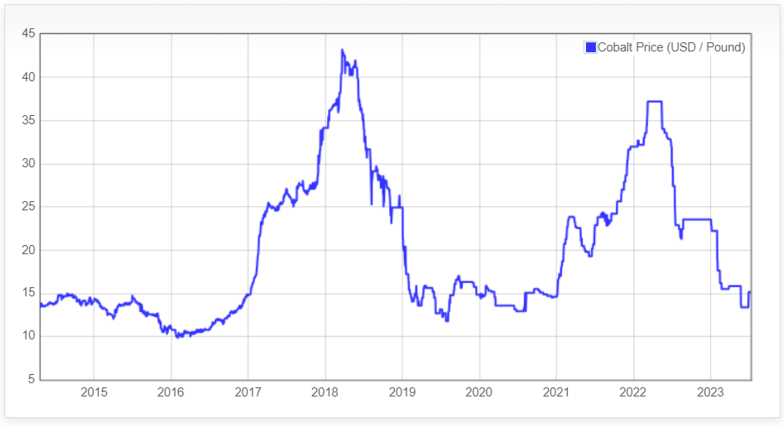
\includegraphics[width=0.7\linewidth]{../images/cobalt_prices}
	\caption{Cobalt prices for the last 10 years}
	\label{fig:cobaltprices}
\end{figure}

\ \\
As a response, on the one hand big mining companies increased their capacity, but on the other hand the artisanal cobalt mining increased, where local people start mining cobalt by themselves. This is however a dangerous and unhealthy practice and can also stimulate child labour. \\
\\
At the same time there were technological improvements to batteries, where they needed almost no cobalt anymore. The increase in supply and smaller increase in demand in turn caused the prices of cobalt to drop again. 
\newpage

\subsubsection{Case: Electric car}

The demand for some metals will increase drastically because of the rapid introduction of electrical vehicles. The question is whether we will not run out of these metals.\\
\\
Nickel as example, needed for the batteries of electrical vehicles, does not suffer from an absolute, nor from a structural scarcity. Yet, the forecasted supply in the coming years is not sufficient to meet the increasing demand when an SDS scenario is pursued. Other actions will be necessary.\\
\\
We also observe a shift in supply towards South-East Asia, potentially strengthening the economic scarcity.

\begin{figure}[H]
	\centering
	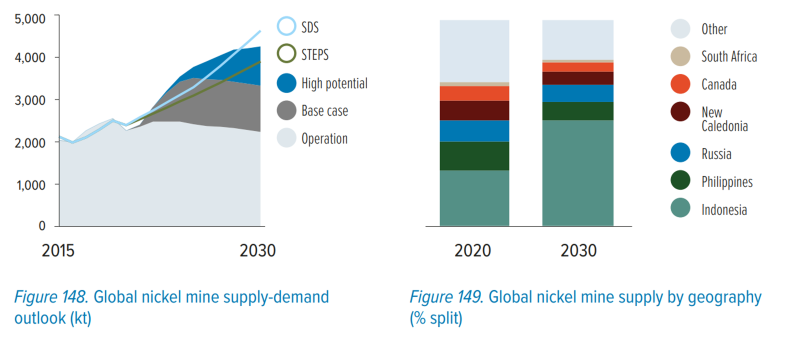
\includegraphics[width=0.8\linewidth]{../images/Global_nickel_supply-demand}
	\caption{Global Nickel supply-demand results}
	\label{fig:globalnickelsupply-demand}
\end{figure}

\subsubsection{Biobased resources}

The scarcity of raw materials is a pressing concern, prompting exploration of solutions, with a significant focus on biobased materials derived mainly from biomass, including trees and cultivated plants. Currently, around one eighth of materials for products are biobased, with 80\% being wood used in construction, furniture, and paper. Innovations in biobased raw materials, especially for replacing fossil-based plastics, are underway. Historically, humans extensively used bio-based materials for tools and clothing until the industrial revolution and the advent of synthetic polymers.\\
\\
Today, there is a growing interest in biobased materials, particularly for plastics. While some are biodegradable, more than half of new biobased plastics are made from "drop-in polymers," mirroring the properties of their fossil-based counterparts. The advantage of biobased raw materials lies in their renewability, provided they are sourced sustainably, considering their regeneration capacity.\\
\\
However, using biobased resources raises several concerns. The cultivation of biomass requires land, leading to potential competition between land use for materials and food production. Intensive land use can deplete soil, impacting biodiversity. Agriculture-related issues like fertilizer and pesticide use contribute to the environmental impact of biobased materials. Water and energy requirements are additional considerations, with some crops needing substantial amounts.\\
\\
The type of biomass source used for biobased materials is evolving. First-generation biomass sources, derived from food crops, raise concerns about competition with food production. Second-generation sources use by-products and waste to avoid this competition. Third-generation sources, extracted from microorganisms like algae, yeasts, and mycelium, eliminate the need for soil.\\
\\
In conclusion, the transition to biobased materials holds promise for replacing non-renewable resources, but a comprehensive investigation into the entire life cycle is necessary to assess and mitigate potential environmental impacts.


\end{document}